\documentclass{llncs}
\usepackage{color}
\usepackage{array}
\usepackage{graphicx}
\usepackage{listings}
  \usepackage{courier}

\begin{document}
%\title{Metashare as an ontology for the interoperability of linguistic datasets}
\title{One ontology to bind them all: The META-SHARE OWL ontology for the interoperability of linguistic datasets on the Web}
%
\titlerunning{META-SHARE ontology} % abbreviated title (for running head)
% also used for the TOC unless
% \toctitle is used
%
% This is not the final order!
%\author{Philipp Cimiano\inst{1} \and Jorge Gracia\inst{2} \and Penny Labropoulou\inst{3} \and John P. McCrae\inst{1} \and V\'ictor Rodr\'iguez Doncel\inst{2} \and Marta Villegas\inst{4}}
\author{John P. McCrae\inst{1} \and Penny Labropoulou\inst{3} \and Jorge
Gracia\inst{2} \and Marta Villegas\inst{4} \and V\'ictor Rodr\'iguez-Doncel\inst{2} \and Philipp Cimiano\inst{1}}
%
\authorrunning{McCrae et al.} % abbreviated author list (for running head)
%
%
\institute{Cognitive Interaction Technology, Excellence Cluster, Bielefeld
University, Germany \\
\email{\{cimiano, jmccrae\}@cit-ec.uni-bielefeld.de}
\and
Ontology Engineering Group, Universidad Polit\'ecnica de Madrid, Spain \\
\email{\{jgracia, vrodriguez\}@fi.upm.es}
\and
ILSP/``Athena'' RC, Athens, Greece \\
\email{penny@ilsp.athena-innovation.gr}
\and
University Pompeu Fabra, Barcelona, Spain \\
\email{marta.villegas@upf.edu}}
\maketitle % typeset the title of the contribution
\begin{abstract}
    META-SHARE is an infrastructure for sharing Language Resources (LRs) where significant effort has been made into
    providing carefully curated metadata about LRs. However, in the face of the flood of data that is used in computational
    linguistics, a manual approach cannot suffice. We present the development of
    the META-SHARE ontology, which transforms the metadata schema used by META-SHARE into ontology in the Web Ontology Language (OWL) that can better handle the diversity of
    metadata found in legacy and crowd-sourced resources. We show how this model can interface with other more general
    purpose vocabularies for online datasets and licensing, and apply this model
    to the CLARIN VLO, a large source of legacy metadata about LRs. Furthermore,
    we demonstrate the usefulness of this approach in two public metadata
    portals for information about language resources.
\keywords{language resources and evaluation, metadata, ontologies, harmonization}
\end{abstract}
\section{Introduction}
\label{sec:introduction}
The study of language and the development of natural language processing (NLP) applications requires access to language resources (LRs). %Lexicographers and terminologists require access to lexical resources and language corpora, corpus linguistics require access to language corpora and developers of natural language processing applications require annotated corporate to train models for part-of-speech tagging, named entity recognition (NER), parsing, etc.
Recently, several digital repositories that index metadata for LRs have emerged,
supporting the discovery and reuse of LRs. One of the most notable of such
initiatives is
META-SHARE\footnote{\url{http://www.meta-share.eu}}~\cite{piperidis2012meta}, an open,
integrated, secure and interoperable exchange infrastructure where LRs are
documented, uploaded, stored, catalogued, announced, downloaded, exchanged and
discussed, aiming to support reuse of LRs. Towards this end, META-SHARE has
developed a rich metadata schema that allows aspects of LRs accounting for their
whole lifecycle from their production to their usage to be described. The schema
has been implemented as an XML Schema Definition (XSD) \footnote{\url{https://github.com/metashare/META-SHARE/tree/master/misc/schema/v3.0}} and descriptions of specific LRs are available as XML documents.

Yet, META-SHARE is not the only source for discovering LRs and their descriptions; other sources include the catalogs of agencies dedicated to the promotion and distribution of LRs, such as ELRA\footnote{\url{http://www.elra.info/en}} and LDC\footnote{\url{https://www.ldc.upenn.edu/}}, other infrastructures such as the CLARIN Virtual Language Observatory (VLO)\footnote{\url{http://catalog.clarin.eu/vlo/?1}}~\cite{broeder2010data}, 
the Language Grid\footnote{\url{http://langrid.org/en/index.html}} and Alveo\footnote{\url{http://alveo.edu.au}}, the Open Language Archives Community (OLAC)\footnote{\url{http://www.language-archives.org}}, 
catalogs with crowd-sourced metadata, such as the LREMap\footnote{\url{http://www.resourcebook.eu/searchll.php}}~\cite{calzolari2012lre}, and, more recently, repositories coming from various communities (e.g. OpenAire\footnote{\url{https://www.openaire.eu/}}, EUDAT\footnote{\url{http://eudat.eu}} etc.). 
%\footnote{Other initiatives aiming to collect and publish information on LRs include Datahub (\url{http://datahub.io/}) which targets datasets published as linked data and the DiRT Directory (\url{http://dirtdirectory.org/}) andTERESAH %!!!!! This URL is obviously not stable, we should update it for the final version!!!!
%(\url{http://staging.teresah.php.dev.dasish.eu/}) focusing on tools for scholars.} 
The metadata schemes of all these sources vary with respect to their coverage and the set of specific metadata captured.
%All these repositories are complementary and index different language resources \textcolor{red}{PL: rephrase: their sources are different but they have overlapping sets of LRs}.
Currently, it is not possible to query all these sources in an integrated and uniform fashion.
The Web of Data is a natural scenario for exposing LRs metadata in order to allow their automated discovery, share and reuse by humans or software agents and the benefits of this model including interoperability, federation, expressivity and dynamicity were laid out by Chiarcos et al.\cite{chiarcos2012towards}.

 %To that end, we have chosen an OWL based representation for the META-SHARE ontology.
In this paper we contribute to the interoperability of these repositories by
developing an ontology in the Web Ontology Language (OWL)~\cite{motik2012owl}
that allows us to represent the metadata schemes of these repositories under an
extensible, open-world model.\footnote{\url{http://purl.org/net/def/metashare}}
%OWL allows for a higher expressive level than the original XML representation as well as the application of semantic reasoning techniques (i.e., to infer new knowledge that were not initially declared). Also, the XML-based representation has proved inefficient when linking metadata resources. In fact, the use of RDF for representing the LRs metadata underlying the OWL ontology enables direct mechanisms for linking between metadata of different LRs and between metadata of LRs and other external sources.
The proposed ontology is based on the ontology developed by Villegas et
al.~\cite{Villegas2014} for the University Pompeu Fabra's (UPF) META-SHARE node (covering part of the original schema), which is extended to the complete schema (in order to cover all relevant LRs) and incorporates the consensus reached in the context of the W3C Linked Data for Language Technologies (LD4LT) Community Group\footnote{\url{https://www.w3.org/community/ld4lt}}.
We show how this model interacts with the DCAT~\cite{maali2014data} vocabulary
as well as the most prominent models in the CLARIN VLO data.
%As a proof of concept of this ontology, we describe how we have mapped metadata records from the above mentioned three repositories (META-SHARE, CLARIN, LRE-Map) into this ontology.
Further, we describe the application of the model in two portals, firstly the
IULA LOD catalogue and secondly
\emph{Linghub}\footnote{\url{http://linghub.org/}}.
%Our approach has several advantages. Firstly, the use of Semantic Web techniques support standardized means of representing, linking, and accessing the data, while 
%(i.e., OWL, RDF) allows us to interlink different LR metadata among themselves and with other external resources on the Web of Data, and enables standardized means of representing and accessing the data (e.g., via SPARQL) thus not relying on domain-specific data formats or proprietary APIs.
%the resulting data is lighter, better suited for exploitation and eases further
%extensions and links with external resources.
%The use of Semantic Web techniques enable standardized means of linking and accessing the data (e.g., via SPARQL) avoiding domain-specific data formats or proprietary APIs.
%In addition, we assume that the use of this ontology will enable the representation of metadata in a manner that allows existing resources to adopt a
%common core vocabulary, while still being able to represent specific extensions
%to their existing model. We evaluate this hypothesis by reference to the 
%CLARIN metadata.

The remainder of this paper is structured as follows: in Section
\ref{sec:relatedwork} we will describe the related work in the fields of
LR metadata harmonization. The development of the
META-SHARE ontology is described in section \ref{sec:ontology}
and its application in Section \ref{sec:applications}.
Finally, in section \ref{sec:conclusion} we consider the broader
impact of this ontology as a tool for computational linguists and as a method to
realize an architecture of (linked) data-aware services.
\section{Related Work}
\label{sec:relatedwork}
The task of finding common vocabularies for linguistics is of wide interest and several general ontologies for linguistics have been proposed. The General Ontology for Linguistic Description~\cite[GOLD]{farrar2002common} was proposed as a common model for linguistic data, but its relatively limited scope and low coherence has not led to wide-spread adoption. An alternative approach that has been proposed is to use ontologies to create coherence among the resources, in particular by using ontologies to align different linguistic schemas~\cite{chiarcos2012ontologies}.

This lack of consensus resides also in the description of LRs, even for non-linguistic concepts. In fact, there are as many metadata schemas for their descriptions as
catalogs and repositories for their presentation (e.g. those used by ELRA and
the LDC) and communities describing them (e.g. TEI~\cite{ide1995text} or
CES~\cite{ide1998corpus}). The most widely used schema for the exchange of LRs is the one  suggested
by the Open Language Archives Community~\cite[OLAC]{bird2001olac}, which builds on
the Dublin Core metadata and has been criticized as being too reductionistic. %~\cite{who} 
%Differences between the schemas lie in the range of features included (e.g. size, technical details, classification etc.), the labels used for the features (e.g. rights, license, policy, terms of use etc. to denote the terms of use for an LR) and the datatypes for the features (e.g. values taken from a closed vocabulary or input as free text). 
Differences between the schemas lie in the range of features used and their labels and datatypes.

An important effort to harmonize metadata has been the ISO Data Category Registry (ISOcat DCR)~\cite{kemps2008isocat}, intended as a registry where metadata providers can register their concepts (Data Categories) and link them to those of other providers. A subset thereof was selected by metadata experts as the core elements for the description of LRs (``Athens Core''). The Component Metadata Infrastructure~\cite{broeder2012cmdi} proposed by CLARIN extends this principle of a common registry to include ``components'' and ``profiles'': ``components'' consist of semantically close elements to be shared among different communities when producing ``profiles'' for specific LR types.
%; however, this has not been achieved (cf. \ref{sec:harmonization}) and the VLO resorts to ISOcat links for aggregating similar resources. 
However, as  we observe in section \ref{sec:harmonization}, this has in practice
merely resulted in each contributing institute using its own scheme, with very
little commonality between different institutes. To improve this situation it
was recently proposed that the conversion of these CMDI schemas to RDF would
enable better interoperability~\cite{durco2014clarin}.

A different approach was taken for the design of the META-SHARE schema ~\cite{gavrilidou2012metashare}, which was based on a comparative study of the most widespread metadata schemas and catalog descriptions, analysis of user needs and discussions with metadata providers and experts in order to arrive at a common schema, taking into account previous initiatives and recommendations (cf. ~\cite{calzolari2010flarenet} and ~\cite{cieri2010metadata}).
%, however it is not clear if this project has been realized.\footnote{JPM: I emailed Menzo Windhouwer about this and may change this statement based on his response, if any; PL: in lrec they said they have rdfized the schemas but there has been no implementation as far as I know; take out unless we're sure}
% Other initiatives aiming to bring together LRs include, among others,
%Datahub\footnote{\url{http://datahub.io/}} which targets datasets published as
%linked data and the DiRT Directory\footnote{\url{http://dirtdirectory.org/}} and
%TERESAH
%!!!!! This URL is obviously not stable, we should update it for the final
% version!!!!
%\footnote{\url{http://staging.teresah.php.dev.dasish.eu/}} focusing on tools for scholars.
%and the Linguistic Linked Open Data \footnote{\url{http://linguistics.okfn.org/resources/llod/}} collecting descriptions of LRs available in Linked Data format.

\section{The META-SHARE OWL Ontology}
\label{sec:ontology}
\subsection{Original MS XSD schema}
\label{sec:xsd}

\begin{figure}
    \centering
    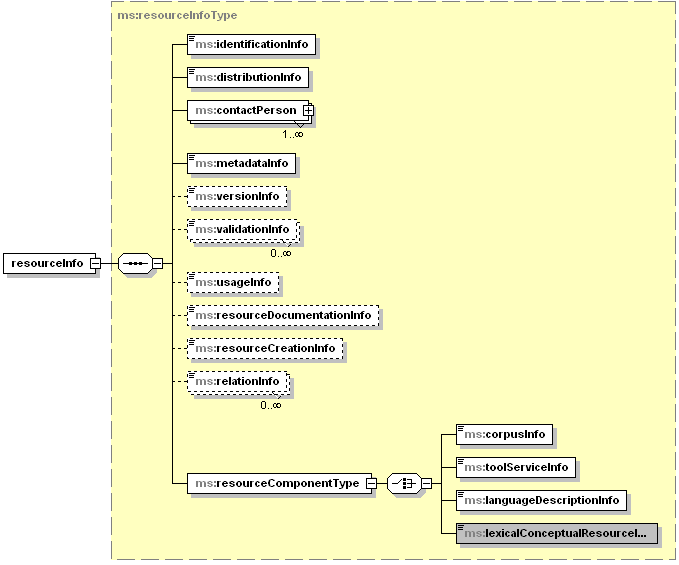
\includegraphics[width=.8\textwidth]{figure_resource.png}
    \caption{\label{fig:resource}The core of the META-SHARE model}
\end{figure}

The META-SHARE schema~\cite{gavrilidou2012metashare} has been designed not only as an aid for LR search and retrieval, but also as a means to foster their production, use and re-use by bringing together knowledge about LRs and related objects and processes, thus encoding information about the whole lifecycle of the LR from production to usage.
The central entity of the META-SHARE schema is the LR \textit{per se}, which
encompasses both {\bf data sets} (e.g., textual, audio and multimodal/multimedia
corpora, lexical data, ontologies, terminologies, computational grammars,
language models) and {\bf technologies} (e.g., tools, services) used for their processing. 
In addition to the central entity, other entities are also documented in the schema; these are reference documents related to the LR (papers, reports,
manuals etc.), persons/organizations involved in its creation and use (creators, distributors etc.), related projects and activities (funding projects,
activities of usage etc.), accompanying licenses, etc., all described with metadata taken as far as possible from relevant schemas and guidelines (e.g. BibTex for bibliographical references). 
The META-SHARE schema proposes a set of elements to encode specific descriptive
features of each of these entities and relations holding between them, taking as
a starting point the LR. Following the CMDI approach, these elements are grouped
together into ``components''. The core of the schema is the {\tt resourceInfo}
component (Figure \ref{fig:resource}), which subsumes: 
\begin{itemize}
\item administrative components relevant to all LRs, e.g. {\tt
    identificationInfo} (name, description and identifiers), {\tt distributionInfo} (licensing and intellectual property rights information), {\tt usageInfo} (information about the intended and actual use of the LR).
\item components specific to the resource type (corpus, lexical/conceptual
    resource, language model, tool/service) and media type (text, audio, video,
    image), which support the encoding of information relevant to resource/media combinations, e.g. text or audio parts of corpora, lexical/conceptual resources etc., such as language, formats, classification.
\end{itemize} 
The META-SHARE schema recognises obligatory elements (minimal version) and recommended and optional elements (maximal version). 
%The META-SHARE schema has been implemented as an XSD (available at {\textcolor{red}{GITHUB}). 
An integrated environment supports the description of LRs, either from scratch or through uploading of XML files adhering to the META-SHARE metadata schema, as well as browsing, searching and viewing of the LRs.
\subsection{Formal modelling and mapping issues}
\label{sec:mapping}

\begin{figure}
    \centering
    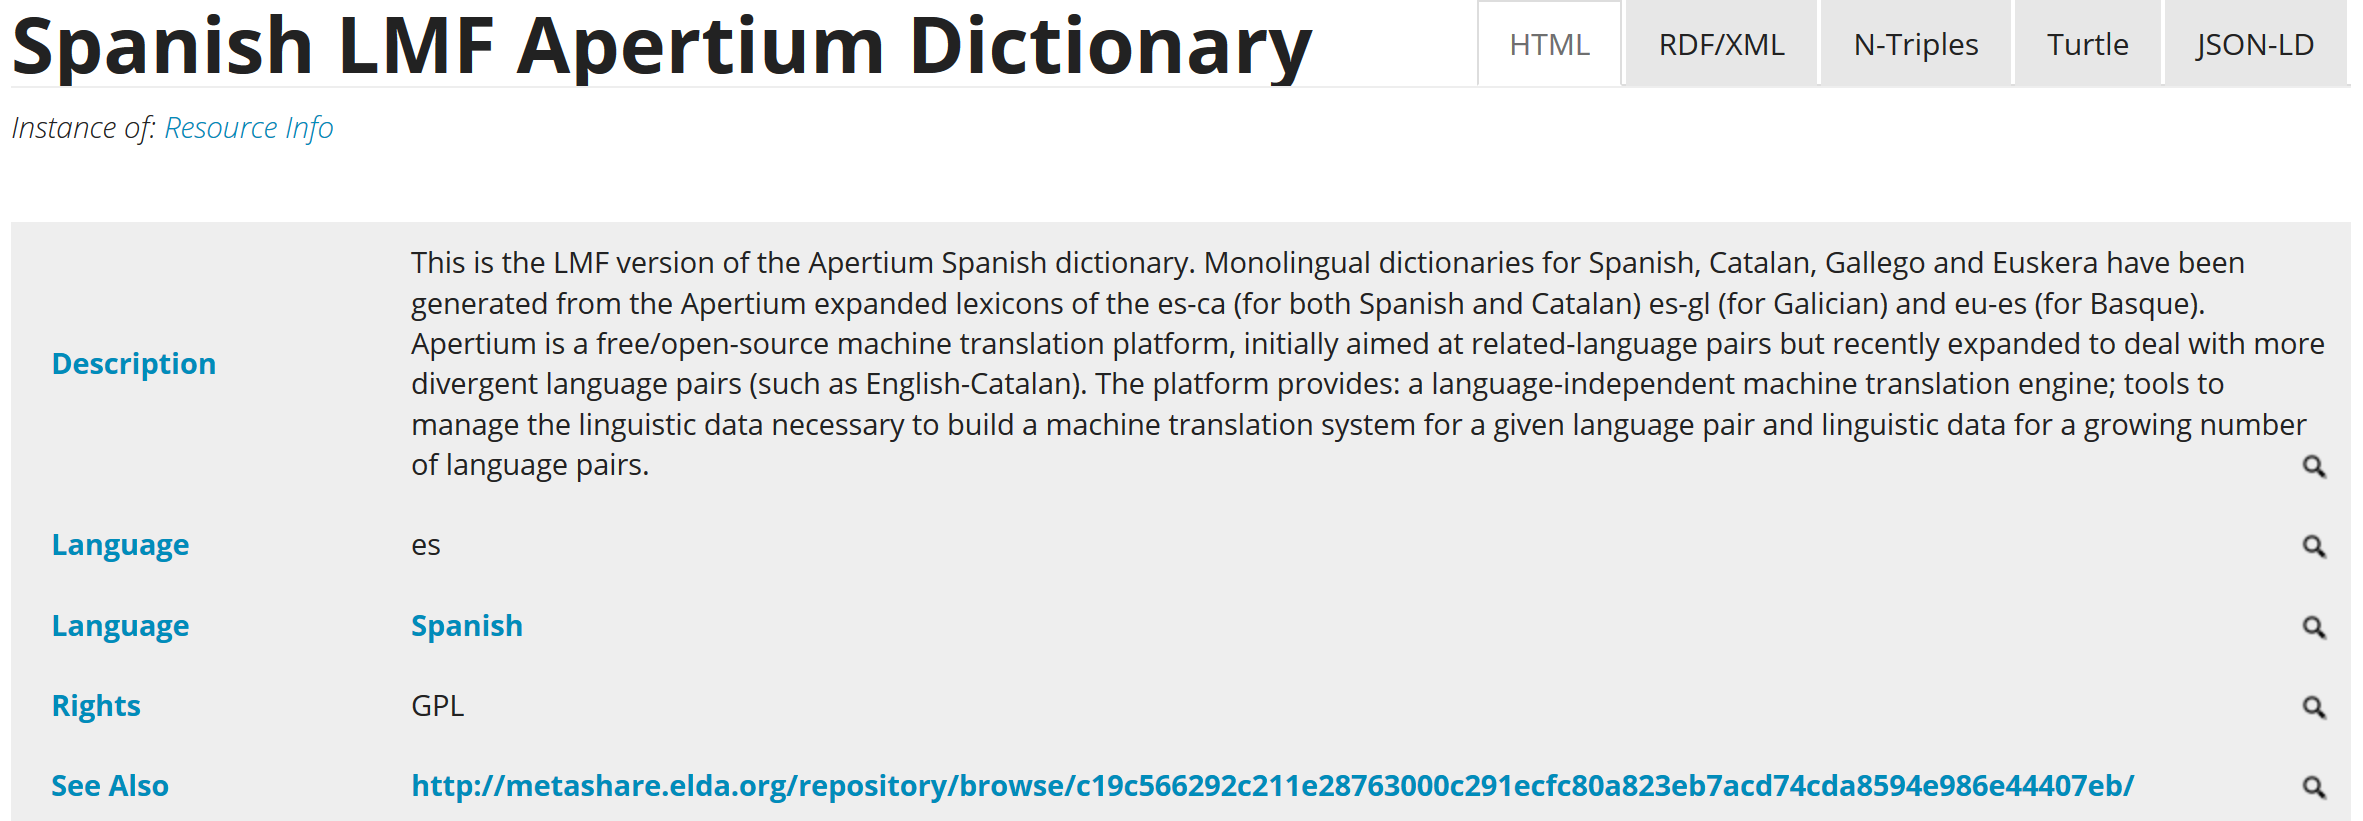
\includegraphics[width=.9\textwidth]{linghub-screenshot.png}
    \caption{META-SHARE data as displayed within the Linghub
    interface\label{fig:screenshot}}
\end{figure}

%{PL: repetition: take out}The META-SHARE metadata model is formalised in a XSD schema that `transcodes' a component-based model as suggested by CLARIN~\cite{broeder2012cmdi}. Essentially, the component-based approach revolves around two central concepts: \emph{elements} and \emph{components}. \emph{Elements} are used to encode specific descriptive features of the resources and are linked to conceptually similar existing elements in the Dublin Core and/or the ISOcat registry. \emph{Components} are complex elements and can be seen as bundle of semantically coherent \emph{elements}.
%{PL: I think this paragraph should be turned into bullets in the list our decisions of mapping, one for the mapping of components/elements and one for the simplification rule}
In the META-SHARE XSD schema, \emph{elements} are formalized as simple elements
whereas \emph{components} are formalized as complex-type elements. When mapping
the XSD schema to RDF, \emph{elements} can be naturally understood as properties
(e.g. name, gender, etc.). \emph{Components} (i.e. complex-type elements),
however, deserve a careful analysis. General mapping rules from XSD to RDF
establish that a local element with complex type translates into an object
property and a class. We observed that the straightforward application of such a
principle may derive unnecessarily verbose graphs. Thus,
following Villegas et al.~\cite{Villegas2014}, we identified potentially removable nodes before
undertaking the actual RDFication process. Embedded complex elements with
cardinality of exactly one are identified as potentially removable, provided they contain
neither text nor attributes. This allows for a simplification of the model, for
example in the chain {\tt resourceInfo} $\circ$ {\tt identificationInfo}
$\circ$ {\tt resourceName}, the {\tt identificationInfo} property is not needed.
Interestingly enough, the removal of the superfluous wrapping elements has also
led to a change of philosophy in the schema and a need for restructuring in order to ensure that properties are attached to the most appropriate node, as exemplified and discussed in Section \ref{sec:licensing}.
Beyond this, we made extensions to our mapping strategy in order to improve the ontology, such as the following:
\begin{itemize}
%\item renaming of elements when falling into one of the following categories:
    \item Removal of the {\tt Info} suffix from the names of  wrapping elements of
        components.
%        , as this makes no sense in the new philosophy of the schema: e.g. {\tt validationInfo} becomes validation (as property) and Validation (as class);
    \item Improvement of names that created confusion, as already noted by the
        META-SHARE group and/or the LD4LT group; thus, {\tt resourceInfo} was renamed
        {\tt LanguageResource}, {\tt restrictionsOfUse} became {\tt
        conditionsOfUse}.
    \item Generalization of concepts, e.g. {\tt
        not\-Available\-Through\-Metashare} with {\tt
        avai\-lable\-Through\-Other\-Distributor};
%    \item avoid duplicates created due to the removal of the Info suffix, as described above, e.g. {\tt characterEncoding} becomes {\tt characterEncodingSet} to differentiate from the property {\tt characterEncoding} (previously {\tt characterEncodingInfo})
\item Development of novel classes based on existing values, for example:
    \\$\mathtt{Corpus} \equiv \exists \mathtt{resourceType}.\mathtt{corpus}$
%\item Movement of properties to other nodes: obviously, when components are removed, the properties are attached to the higher node; but also for cases where there's a change of concept, as described in \ref{sec:licensing} 
\item Grouping similar elements under novel superclasses, e.g. {\tt
    annotationType} and {\tt genre} values are structured in classes and
    subclasses better reflecting the relation between them. Indicatively, the superclass
    {\tt SemanticAnnotation} can be used to bring together semantic annotation types,
    such as semantic roles, named entities, polarity, and semantic relations.
\item Extension of existing classes with new values and new properties
    (e.g. {\tt licenseCategory} for licences).
\end{itemize}

The actual mapping was achieved by means of a custom domain-specific language
inspired by XML Stylesheet Transforms.

\subsection{Interface with DCAT and other vocabularies}

\begin{figure}
    {\footnotesize
    \begin{verbatim}
<> a dcat:Dataset ;
  dc:description "Cette base de données..."@fr
  dc:language "tur" ;
  dc:source "META-SHARE" ;
  ms:corpusInfo <#corpusInfo> ;
  ms:distributionInfo <#distributionInfo> ;
  rdfs:seeAlso <http://metashare.elda.org/reposit...ac770/> .

<#corpusInfo> a ms:CorpusInfo , ms:CorpusAudioInfo ;
  dc:language "tur" ;
  ms:languageName "Turkish" ;
  ms:mediaType ms:audio .

\end{verbatim}}
\caption{An abridged example of a metadata entry represented with common metadata
    properties from DCAT and Dublin Core and novel properties from the MetaShare
ontology.\label{fig:example-dcat}}
\end{figure}

\label{sec:dcat}
The META-SHARE model can be considered broadly similar to DCAT in that there are
classes that are nearly an exact match to the ones in DCAT for three out of four
classes. DCAT's {\tt dataset} corresponds nearly exactly to the {\tt resourceInfo} tag and, similarly, {\tt distributions} are similar to {\tt distributionInfo} 
classes and {\tt catalogRecord} is similar to {\tt metadataInfo}. Thus, we
introduced \emph{equivalent class} relations between these elements. The
fourth main class, {\tt catalog} covers a level not modelled by META-SHARE.
DCAT uses Dublin Core properties for many parts of the metadata, and often these
properties are found deeply nested in the META-SHARE description. For example, language
is found in several places deeply nested under six
tags\footnote{e.g., {\tt resourceInfo} $\circ$ {\tt resourceComponentType}
    $\circ$ {\tt corpus} $\circ$ {\tt corpusMediaType} $\circ$ {\tt corpusVideoInfo}
    $\circ$ {\tt
languageInfo} $\rightarrow$ {\tt dc:language}}. In META-SHARE this allows different media types in the resource
to have different languages, e.g., the dialogues and the scripts of a video may
be in English, whereas the subtitles can be in French and German.
We still include this fine-grained metadata but also add the property at the resource level
to indicate if any part of the resource is in the stated language.
%This is in accordance to the META-SHARE view that a language resource may consist of modules with different media types, which have different properties and need to be described in different terms: for instance, a multimedia corpus may have a video module (the moving image part per se), a video module for the dialogues which can be separated from the video, and three text modules for the subtitles, the transcription of the dialogues and the scripts. These modules can have different properties, e.g. the dialogues and the scripts may be in English, but the subtitles can be in French and German (two translations). Thus, language as a property is attached not to the languageResource but to each module. Even after removing the superfluous nodes, language will still be embedded at a deeper level, although not as deep as in the XSD schema.
Similarly, it is also the case that some Dublin Core properties are not directly
specified in the META-SHARE model, but can be inferred from related properties,
e.g., Dublin Core's `contributor' follows (by means of a property chain) from people indicated as `annotators',
`evaluators', `recorders' or `validators'. Furthermore, several DCAT specific-properties, such as `download URL', are nearly
exactly equivalent to those in META-SHARE but occur in places that do not fit the
domain and range of the properties. In this particular case, it was a simple fix
to move the property to the enclosing {\tt DistributionInfo} class.
Inevitably, several properties from DCAT did not have equivalences in
META-SHARE, notably `keyword'.

In addition to DCAT, we used also other vocabularies to establish equivalences to parts of the model. In particular, we mapped to the Friend of
a Friend (FOAF) ontology to describe people and organizations and the Semantic
Web for Research Communities (SWRC) ontology to describe scientific
publications.

\subsection{Licensing module}
\label{sec:licensing}

A specific area where we made a significant effort to improve the modelling was
in the licensing information in order to allow the formulation of a clear and
concise rights information of the LRs. 
Some languages already exist for this purpose and, among them, ODRL 2.1 (Open Digital Rights Language) was
chosen and extended. ODRL is a policy and rights
expression language specified by the W3C ODRL Community
Group\footnote{\url{https://www.w3.org/community/odrl/}}, which defines a model
for representing permissions, prohibitions and duties.
The most common licenses (for software, data or general works) have been already
expressed in ODRL in the RDF License dataset~\cite{rdflicense} and can be pointed to when an LR is licensed with any of these.
Extensions to the ODRL vocabulary have been made to represent some of the specificities
of the LR domain. The specification also suggested changes, some of them
structural, to the previous META-SHARE modelling, and to this extent we
combined the existing META-SHARE licensing vocabulary with ODRL.
In addition, we extended the model by adding some new properties and individuals
based on requirements from the LD4LT community group\footnote{\url{https://www.w3.org/community/ld4lt/wiki/Metashare\_vocabulary\_for\_licenses}}.
%META-SHARE limits fuzziness in the terms and conditions of use of LRs by
%providing a range of recommended standard licenses organized on the following axes: open licenses are the preferred option (Creative Commons licenses %for data resources and Free Open Source Software for tools and
%services), followed by two sets of model (standard) licenses built in response
%to LR providers' requests (META-SHARE Commons and NoRedistribution licenses);
%custom and proprietary licenses are also allowed for legacy
%resources that cannot be licensed otherwise. 
In particular, the generic \textit{conditions-of-use} values of the META-SHARE schema have been exploited for
creating RDF codes for non-standard licenses and are mapped to ODRL
actions (e.g. the duty to attribute), and included in an RDF
document, as shown in Figure \ref{fig:license-example}.
%Extension with more variable aspects of licenses can be added on top. In this way, some of the variable
%elements are detached and more easy editable. 
This module has been published both as independent module\footnote{\url{http://purl.org/NET/ms-rights}} 
and as part of the META-SHARE ontology. 
%An example on how language resources can be licensed is shown by the RDF document below: a resource is offered under one of the META-SHARE recommended licenses: the Meta-Share Commercial-NoRedistribution-ForAFee license. This is a generic license template published online, whose precise fields (parties, specific price) are in blank. This license offers a resource for a free and forbids its redistribution.

\begin{figure}
\begin{verbatim}

<#distributionInfo> a ms:DistributionInfo , dcat:Distribution ;
  dct:license <http://purl.org/NET/rdflicense/ms-c-nored-ff> ;
  dcat:accessURL <http://catalog.elra...> .
\end{verbatim}
\caption{An example of the modelling of licenses in a record\label{fig:license-example}}
\end{figure}

%A Dublin Core license property links the resource with the license, and the price -whose precise number is not specific in the generic license online- is given using the GoodRelations\footnote{\url{http://www.heppnetz.de/projects/goodrelations/}} vocabulary. The RDF version of this generic license can also be found online, in a structure that permits some degree of reasoning on the licensing terms. 

%These changes included the selection of classes and properties from other existing vocabularies (specifically from ODRL, Dublin Core, Creative Commons REL\footnote{\url{http://creativecommons.org/ns}} and SKOS) as well as the definition of new ones.

%One of the most important achievements of META-SHARE has been the formulation of a clear, consise and easy-to-use licensing model to specify the rights information of the LRs. 
%%Licensed LRs can be shared and re-used with legal guarantees complying with the statement of the META-SHARE Charter\footnote{\url{http://http://www.meta-net.eu/meta-share/METASHARE\_Charter.pdf}}: ``\textit{LRs should be shared and further re-used with the minimum possible transaction costs and efforts and under clear and easy to understand rules}''. This is of high importance since the production of LRs of good quality and quantity, as required for the research and development of Language Technology, is cost- and time-consuming and only their sharing and re-use can render them cost-effective.
%%{PL: to shorten the section, this could be left out}LR are sometimes offered under a well-known license (e.g. Creative Commons, CC), and sometimes under the specific terms and conditions declared by the rightsholder; they are sometimes open\footnote{We consider \textit{open licenses} to be those that include not only the right to read the relevant content but also to allow transformative uses, dissemination and distribution of such resources and their derivatives, according to the needs and policies of LR owners and users.} and sometimes offered under more limiting conditions.
%%This principle has been shaped in the form of a set of legal documents, guidelines and recommendations supporting LR providers in licensing their LRs.
%%Moreover, LR consumers need to know precisely what they can do with an LR without asking the help of legal experts. 
%%The rights information of these LRs should be expressed in an uniform and coherent manner, so that users and machines alike can process the information.
%
%%http://www.essepuntato.it/lode/http://www.essepuntato.it/tmp/1425385313-ontology#objectproperties
%
%In order to limit fuzziness in the terms and conditions of use of LRs, META-SHARE recommends the use of standard licenses (preferably open ones); while proprietary or closed licenses and texts with terms of use are to be avoided. Moreover, the metadata schema includes a module on licensing, which forces LR providers to document the conditions of use of their resources in a standardised format. Elements in the module encode rights holders, the most frequently used conditions and terms (e.g. attribution, no derivatives etc.), formats and location of the distribution files, pricing details etc., while the licence itself is obligatorily selected from a list of predefined values representing the recommended licences.
%
%%The mechanism for implementing this set of recommendations has been the metadata module on licensing, which forms an essential ingredient of the schema. The elements describing rights of use and distribution details are included in the obligatory component {\tt distributionInfo} and its embedded {\tt licenceInfo}, i.e. all LRs documented in META-SHARE include obligatorily a description on their conditions of use in a standardised format. The schema contains specific elements for:
%%\begin{itemize}
%%\item the distribution and use conditions, including {\tt licence} with links to the recommended licences, elements such as {\tt conditionsOfUse} which  comprises a list of the most frequent terms and conditions of use associated with LRs, eg. noDerivatives, nonCommercialUse, attribution etc. and can be used as a quick guide for human users to understand what they can and cannot do with a resource, and elements for the more detailed information required by specific conditions of use, i.e. {\tt fee} for LRs offered with a monetary compensation, {\tt attributionText} for those requiring attribution, etc.
%%\item rights holders (e.g. {\tt iprHolder}, {\tt distributionRightsHolder})
%%\item distribution information, i.e. the medium and url (if available over the internet) from which the LR is distributed.
%%\end{itemize}
%%Optionality and cardinality are specified for each element/component: {\tt licence} is obligatory for all available LRs and the component {\tt licenceInfo} can be repeated to cater for LRs that are offered with multiple licences, e.g. for commercial purposes with a fee and for research for free.
%
%In the conversion of META-SHARE from XSD to OWL/RDF, we decided to replace the components with classes that can be used to better represent the licensing ecosystem of LRs, and to re-structure the elements in order to make clearer the properties associated with them. As a result, we recognize the following three entities/classes, each associated with different properties as appropriate:
%\begin{itemize}
%\item \verb|LanguageResource|, which is the intellectual property \textit{work}, can be attributed with the \verb|iprHolder| and the \verb|distributionRightsHolder|;
%\item \verb|Distribution|, taken from the DCAT vocabulary where it "\textit{represents an accessible form of a dataset as for example a downloadable file, an RSS feed or a web service that provides the data}"; this is the entity to where licensing information, forms and other details are attached;
%\item \verb|License|, with the specific information that can help us generalize over terms and conditions and enriched with concepts from the ODRL ontology.
%\end{itemize}
%
%Terms and conditions of use can be declared by using URIs pointing to the legal text (or a human readable version) of well-known licenses or to a URL with the specific terms of the LR provider. However, this practice does not favour automated processing and the rights information thus referred would not be queriable. In order to overcome this, a fine-grained representation of licenses, where the specific rights and conditions are given in RDF, was decided. 
%Some languages already exist for this purpose, and among them, ODRL 2.1 was chosen and extended. ODRL (Open Digital Rights Language) is a policy and rights expression language specified by the W3C ODRL Community Group\footnote{\url{https://www.w3.org/community/odrl/}} which defines a model for representing permissions, prohibitions and duties, as well as a core vocabulary. 
%%The abstract model can be serialized as JSON, XML or RDF, the latter option being supported by the ODRL 2.1 Ontology\footnote{\url{http://www.w3.org/ns/odrl/2/}}. 
%
%Extensions to the vocabulary were needed to represent some of the specificities of the LRs domain. The specification and led to changes, some of them structural, with respect to the previous versions. These changes included the selection of classes and properties from other existing vocabularies (specifically from ODRL, Dublin Core, Creative Commons REL\footnote{\url{http://creativecommons.org/ns}} and SKOS) as well as the definition of new ones.
%In addition, the recommended standard licenses have been represented in ODRL and published\footnote{\url{http://purl.org/NET/ms-rights}} of the RDF resources to describe licenses was based on a list of requirements\footnote{\url{https://www.w3.org/community/ld4lt/wiki/Metasharevocabularyforlicenses}}. Further, as a support for the representation of non-standard licences (that has to be done by Semantic Web laymen), the new concept of \textit{license templates} has been proposed. A license template is an RDF document with common terms and conditions (e.g. attribution) mapped to ODRL actions (duty to attribute) which are ready to be complemented by other information that changes more frequently. In this way, some of the variable elements are detached and more easy editable.
\subsection{Harmonizing other resources with META-SHARE}
\label{sec:harmonization}
%The LingHub portal indexes metadata from a wide-range of sources. 
While a basic level of interoperability can be established by using standard
vocabularies such as DCAT and Dublin Core, this can only be done by sacrificing
completeness and ignoring all metadata particular to language resources. For
this reason, we use the META-SHARE model to represent and harmonize the metadata
relating specifically to the domain of linguistics and language resources. As a
proof-of-concept, we show how the META-SHARE ontology supports the harmonization
of data from the CLARIN VLO. The
CLARIN repository describes its resources using a small common set of metadata
and a larger description defined by the Component Metadata
Infrastructure~\cite[CMDI]{broeder2012cmdi}. These metadata schemes are
extremely diverse as shown in Table \ref{tab:clarin-types}.
We will focus on the
top five of these types for which we have created corresponding mappings. Two of these schemes are only Dublin Core properties and so do not have
specific language resource metadata. The most frequent tag 'Song' is used to describe records of a 
database consisting of musical recordings. While many of the properties used by this tag (e.g., `number of
stanzas') have no correspondence in Dublin Core, they can be described with respect to existing elements of the META-SHARE Ontology.
%through properties to describe 
%the technical format information (i.e., `audio
%encoding'). 
The {\tt Session} tag is used to provide IMDI metadata~\cite{broeder2001imdi}, and has a very loose correspondence to META-SHARE. For instance, there are no corresponding properties to describe the participants of a media recording.
This highlights the advantage of
taking an open world, ontological approach as opposed to a fixed schema, in that
we can easily introduce new properties while still reusing the META-SHARE properties
where they are appropriate.
The MODS metadata
scheme~\cite{gartner2003mods} is in fact a general domain metadata framework.
We found that 28 entities from META-SHARE
corresponded to elements used in the `Sing' metadata of the Meertens Institute collection, and 37 to the IMDI metadata,
although there was only minor overlap with the MODS scheme (in particular 4
entities used to describe language) as this scheme is not specific to language
resources.

\begin{table}
\begin{center}
\begin{tabular}{l|lc}
Component Root Tag & Institutes & Frequency \\
\hline
Song & 1 (MI) & 155,403 \\
Session & 1 (MPI) & 128,673 \\
OLAC-DcmiTerms & 39 & 95,370 \\
MODS & 1 (Utrecht)& 64,632 \\
DcmiTerms & 2 (BeG,HI) & 46,160 \\
SongScan & 1 (MI) & 28,448 \\
media-session-profile & 1 (Munich) & 22,405 \\
SourceScan & 1 (MI) & 21,256 \\
Source & 1 (MI) & 16,519 \\
teiHeader & 2 (BBAW, Copenhagen) & 15,998 \\
\end{tabular}
\end{center}
\caption{\label{tab:clarin-types}The top 10 most frequent component types in
CLARIN and the institutes that use them. Abbreviations: MI=Meertens Institute (KNAW),
MPI=Max Planck Insitute (Nijmegen), BeG=Netherlands Institute for Sound and Vision,
HI=Huygens Institute (KNAW), BBAW=Berlin-Brandenburg Academy of Sciences}
\end{table}
\section{Applications}
\label{sec:applications}
\subsection{IULA LOD Catalogue}
\label{sec:iulalod}
The IULA-UPF CLARIN Competence
Centre\footnote{http://www.clarin-es-lab.org/index-en.html} aims to promote and
support the use of technology and text analysis tools in the Humanities and
Social Sciences research. The centre includes a
Catalogue\footnote{http://lod.iula.upf.edu/} with information on language
resources and technology. The Catalogue is based on the initial linked open data
(LOD) version of the META-SHARE model as described in~\cite{Villegas2014} and
the original data originate from the UPF META-SHARE
node\footnote{http://metashare.upf.edu}. The source XML records were converted
into RDF and augmented with service descriptions (not included in the UPF
META-SHARE node) and relevant documentation (appropriate articles,
documentation, sample data and results, illustrative experiments, examples from
outstanding projects, illustrative use cases, etc) to encourage potential users
to embrace digital tools. Finally, the data was enriched with internal and
external links. The resulting linked data maximised the information
contained in the original repository and enabled data mashup techniques that get
relevant data from the DBpedia and the
DBLP\footnote{http://dblp.uni-trier.de/db/index.html}. The catalogue
demonstrates the benefits of the LOD framework and how this can be easily used
as the basis for a web browser application that maximizes information and helps
users to navigate throughout the datasets in a comprehensive way.
\subsection{Linghub}

Linghub is a portal designed to allow common querying of metadata from multiple
highly heterogeneous repositories. Currently, it draws not only
from META-SHARE, but also from the LRE-Map~\cite{calzolari2012lre}, the CLARIN
VLO~\cite{broeder2010data} and DataHub, and is regularly updated with new/changed information. The repository is based on the DCAT and Dublin Core vocabularies. However, these models do not capture
any specific linguistic information. For this reason, the ontology described in this paper is currently being integrated into the system to allow users to use META-SHARE as the
basic vocabulary for querying linguistic information about language resources, and the mappings previously
described have already been applied to data from LRE-Map and the CLARIN VLO.
Linghub supports browsing and querying by several means, including faceted
browsing, full-text search, SPARQL querying and related item search. As such, we
believe that the portal, while not a direct collector of metadata, will enable
users to find more language resources and do so more easily.
The Linghub portal is thus a proof-of-concept for the level of
harmonization that the use of a common ontology provides, as metadata
originating from different repositories can be uniformly queried in Linghub in
an integrated fashion. We adhere to an open architecture in which not only
Linghub but other discovery services that aggregate and index data could potentially
be developed.


\section{Conclusion}
\label{sec:conclusion}
This work represents only a first starting point for the harmonization of
language resources by providing a standard ontology that can be used in the
description of metadata of linguistic resources
and there are still a number of challenges
ahead of us to be addressed. Firstly, the next step would be to make sure that
not only metadata, but the actual data is available on the Web in open web
standards such as RDF so that data can be automatically crawled and analyzed.
Secondly, it should be required that linguistic data published on the
Web should ideally follow the same format (e.g. RDF) so that it can be
easily integrated and data can be queried across datasets. This presupposes
the agreement on best practices for data publication and formats, and the
Natural Language Processing Interchange Format
(NIF)\cite{hellmann2013integrating} is an obvious candidate for that. Thirdly,
harmonization should be extended to the description of NLP services so that NLP
services can be distributed across providers and repositories. The mechanisms for
description of the functionality of NLP services should be extremely
light-weight. Finally, input and output formats for services should be
standardized and homogenized so that services can be easily composed to realize
more complex workflows, without relying on too much parametrization. Workflows
of services should be easily executable \emph{`on the cloud'}. In order to
scale, services should support parallelization, streaming and 
non-centralized processing. %Service execution and composition should not require
%special libraries, grids or other proprietary infrastructures or protocols, but
%rely only on open web standards and protocols such as the hypertext transfer
%protocol (HTTP) and content negotiation, ideally being RESTful to keep APIs
%simple and stateless. 
We believe that the development of common vocabularies
such as the one presented in this paper should enable the emergence of a new paradigm supporting the discovery and exploitation of linguistic data and services across repositories.


\subsubsection*{Acknowledgments.} We are very grateful to the members of the W3C Linked Data for Language Technologies (LD4LT) for all the useful feedback received and for allowing this initiative to be developed as an activity of the group. This work is supported by the FP7 European project LIDER (610782), by the Spanish Ministry of Economy and Competitiveness (project TIN2013-46238-C4-2-R and a Juan de la Cierva grant), the Greek CLARIN Attiki project (MIS 441451) and the H2020 project CRACKER (645357).
\bibliographystyle{splncs03}
\bibliography{metashare-ontology-msw4}
\end{document}
